\documentclass{aa}
% \documentclass[referee]{aa}
\usepackage[varg]{txfonts}
\usepackage[separate-uncertainty=true]{siunitx}
\usepackage[version=3]{mhchem}

\sisetup{range-units = brackets}

\def\eps{\varepsilon}
\def\aap{A\&A}
\def\eprint{e-prints}
\def\apj{ApJ}
\def\apjs{ApJS}
\def\apjl{ApJL}
\def\mnras{MNRAS}
\def\aj{AJ}
\def\nat{Nature}
\def\aaps{A\&A Supp.}
\def\prd{Phys. Rev. D}
\def\prl{Phys. Rev. Lett.}
\def\araa{ARA\&A}

\begin{document}


\title{High resolution near-IR spectroscopy of Arcturus and 10 Leo}
\subtitle{Refining a near-IR iron line list}


\author{ D.~T.~Andreasen\inst{1,2}
    \and S.~G.~Sousa\inst{1}
    \and E.~Delgado Mena\inst{1}
    \and N.~C.~Santos\inst{1,2}
    \and T.~Lebzelter}


\institute{
Instituto de Astrof\'isica e Ci\^encias do Espa\c{c}o, Universidade do Porto, CAUP, Rua das Estrelas, 4150-762 Porto, Portugal
\email{daniel.andreasen@astro.up.pt}
\and
Departamento de F\'isica e Astronomia, Faculdade de Ci\^encias, Universidade do Porto, Rua Campo Alegre, 4169-007 Porto, Portugal
\and
Departamento de F\'{i}sica, Universidade Federal do Rio Grande do Norte, 59072-970 Natal, RN, Brazil
}





\date{Received ...; accepted ...}

\abstract
% Context
{Effective temperature, surface gravity, and metallicity are basic
spectroscopic stellar parameters necessary to characterize
a star or a planetary system. Reliable atmospheric parameters for
FGK stars have been obtained mostly from methods that relay on high
resolution and high signal-to-noise optical spectroscopy. The
advent of a new generation of high resolution near-IR spectrographs
opens the possibility of using classic spectroscopic methods with
high resolution and high signal-to-noise in the NIR spectral window.}
% Aims
{tralala}
% Methods
{Our spectroscopic analysis is based on the iron excitation and ionization
balance done in LTE. We use a high resolution and high signal-to-noise ratio
spectrum of the Sun from the Kitt Peak telescope as a starting point to compile
the iron line list. The oscillator strengths ($\log\mathit{gf}$) of the iron
lines were calibrated for the Sun. The abundance analysis was done using the
MOOG code after measuring equivalent widths of 357 solar iron lines.}
% Results
{tralala}
% Conclusions
{}



\keywords{data reduction: high resolution spectra --
          stars individual: Arcturus --
          stars individual: 10 Leo}
\maketitle



\section{Introduction}
\label{sec:introduction}

Effective temperature ($T_\mathrm{eff}$), surface gravity ($\log g$),
and metallicity ([M/H], where iron is normally used as a proxy)
are fundamental atmospheric parameters necessary to characterise a single
star, and to determine other indirect fundamental parameters
such as mass, radius, and age from stellar evolutionary models
\citep[see e.g.][]{Girardi2000,Dotter2008,Baraffe2015}.
Precise and accurate stellar parameters are also essential in
exoplanet searches. Planetary radius and mass are mainly found from
lightcurve analysis and radial velocity analysis, respectively. The
determination of the mass of the planet implies a knowledge of the
stellar mass, while the measurement of the radius of the planet
is dependent on our capability to derive the radius of the star
\citep[see e.g.][]{Torres2008,Ammler2009,Torres2012}.

The derivation of precise stellar atmospheric parameters is not a simple task.
Different approaches often lead to discrepant results
\citep[see e.g.][]{Santos13}. Interferometry is usually considered  an accurate
method for deriving stellar radii \citep[e.g.][]{Boyajian2012}; however, it is
only applicable for bright nearby stars. Asteroseismology, on the other hand,
reveals the inner stellar structure by observing the stellar pulsations at the
surface. From asteroseismology it is possible to measure the surface gravity and
mean density, and therefore to calculate the mass and radius
\citep[e.g.][]{Kjeldsen1995}.

A crucial parameter for the indirect determination of stellar bulk
properties is the effective temperature. In that respect, the infrared
flux method (IRFM) has proven to be reliable for FGK dwarf and
subgiant stars. However, the IRFM needs a priori knowledge of the
bolometric flux, reddening, surface gravity, and stellar metallicity
\citep{Blackwell1977,Ramirez2005b,Casagrande2010}.

Finally, the use of high resolution spectroscopy along with stellar atmospheric
models is an extensively tested method that allows the derivation of the
fundamental parameters of a star \citep[see e.g.][]{Valenti2005,Santos13}. The
procedure depends on the quality of the spectra, their resolution, and
wavelength region. For low resolution spectra ($\lambda/\Delta\lambda <
20\,000$) the preferred method is to fit the overall observed spectrum with a
synthetic one \citep[see e.g.][]{Recio2006}. Higher resolution spectra of slowly
rotating stars (below 10 to 15 \si{km/s})  are in the regime where the
equivalent width (EW) method can be used
\citep[see e.g.][for details]{Andreasen2017a}.

The derivation of stellar atmospheric parameters from high resolution spectra in
the optical is now based on a standard procedure
\citep[see e.g.][]{Valenti2005,Sousa2008a}. With the advancement of high
resolution near-infrared (NIR) instruments, we will now be able to use a similar
technique to that used in the optical part of the spectrum
\citep[see e.g.][]{Melendez1999,Sousa2008a,Tsantaki2013,Mucciarelli2013,Bensby2014}.
At the moment, the GIANO spectrograph installed at \emph{Telescopio Nazionale
Galileo} (TNG) is already available \citep{GIANO}, the \emph{infrared Doppler
instrument} (IRD) installed at the Subaru telescope \citep{IRD}, as is
\emph{Calar Alto high-Resolution search for M dwarfs with Exoearths with
Near-infrared and optical Échelle Spectrographs} (CARMENES) for the \SI{3.5}{m}
telescope at Calar Alto Observatory \citep{CARMENES}. Two new spectrographs are
planned for the near future: 1) The \emph{CRyogenic InfraRed Echelle
Spectrograph Upgrade Project} (CRIRES+) at the \emph{Very Large Telescope} (VLT)
\citep{CRIRESp} with expected first light in 2017, and 2) \emph{un
SpectroPolarimètre Infra-Rouge A Near-InfraRed Spectropolarimeter} (SPIRou) at
\emph{The Canada-France-Hawaii Telescope} (CFHT) \citep{SPIROU1,SPIROU2} with
expected first light in 2017 as well. The spectral resolutions for these
spectrographs range between $50\,000$ and $100\,000$.

With the advance of NIR spectrographs, we are yet to be to ready for the
analysis of the data arriving at the moment and in the future. The analysis of
stellar spectra is well understood for FGK stars in the optical part of the
spectrum, however some work still needs to be done for the NIR part.

In this work we analyse the atlas of Arcturus (K0III) and the spectrum 10 Leo
(K1III). The atlas of Arcturus was acquired at Kitt Peak National Observatory
using the FTS spectrograph at the Mayall telescope \citep{Hinkle2003} and 10 Leo
from CRIRES \citep{Nicholls2016}. For the analysis we use the iron line list
presented in \citet{Andreasen2016}. This work serve as a continuation of our
previous work.

The paper is organized as follows. In Sect.~\ref{sec:data} we present the data
we have acquired for this work along with some information of the two stars we
will analyse. in Sect.~\ref{sec:refining_the_line_list} we refine the iron line
list in order to get more reliable stellar parameters. The results are presented
in Sect.~\ref{sec:results} before we discuss our results in
Sect.~\ref{sec:conclusion}.




\section{Data}
\label{sec:data}

While the community is currently on the verge to access of a large amount of
high resolution NIR spectra with e.g. the spectrographs used here, the available
spectra at the moment are sparse. We chose to use two stars cooler than the Sun
since we showed in \citet{Andreasen2016} that this method works for a star
hotter than the Sun (HD20010).

We have collected the atlas of Arcturus, one of the brightest stars on the
Northern hemisphere. Thus it is well studied
\citep[see e.g.][to mention a few]{Griffin1967,McWilliam1990,Ramirez2013}. We
use the atlas from \cite{Hinkle2003} which covers the spectral range of interest
(YJHK bands). Strong telluric features were identified with a spectrum from the
TAPAS web page \citep{Bertaux2014}. The atlas also comes with the telluric from
a telluric standard and the ratio of the two spectra in order to correct for the
tellurics. We use both, but note that the telluric correction for Arcturus is
not of the same quality as for 10 Leo as described below.

The second spectrum we have achieved is from the CRIRES-POP team
\citep{Nicholls2016}. 10 Leo is a very similar star to Arcturus, which is also
one reason this star was the first to be fully reduced by the team. It is a
great help to be able to compare with the atlas of Arcturus. The main difference
is the metallicity of the two stars, where Arcturus is metal poor and 10 Leo has
solar metallicity. due to a telluric that could not be properly removed, low
S/N, bad pixels, etc. Rather than giving an uncertain interpolation,
\citet{Nicholls2016} decided to leave small gaps in the data. This have very
little affect on this analysis. However, we were unable to measure one
\ion{Fe}{II} line, which are very important to determine the surface gravity.

A small summarise of the data is given in Tab.~\ref{tab:data}. The data is very
similar, with similar S/N which is an approximately value measured with IRAF.
The resolutions of the two spectrographs used are the same.


\begin{table*}[htb!]
    \caption{The spectra and spectral type (from Simbad) of our sample with
             the corresponding spectrograph used to acquire the data and its
             spectra resolution. In the last column we show the S/N measured
             with splot in IRAF.}
    \label{tab:data}
    \centering
    \begin{tabular}{lrrrr}
      \hline\hline
        Star      & Spectral type & Spectrograph  & Resolution   &  S/N  \\
      \hline
        Arcturus  &      K0III    & FTS           &  $100\;000$  &  300  \\
        10 Leo    &      K1III    & CRIRES        &  $100\;000$  &  300
    \end{tabular}
\end{table*}


In Fig.~\ref{fig:both} we compare the spectra of the two stars in a region with
some of the iron lines used for the analysis described below.

\begin{figure*}[tpb]
    \centering
    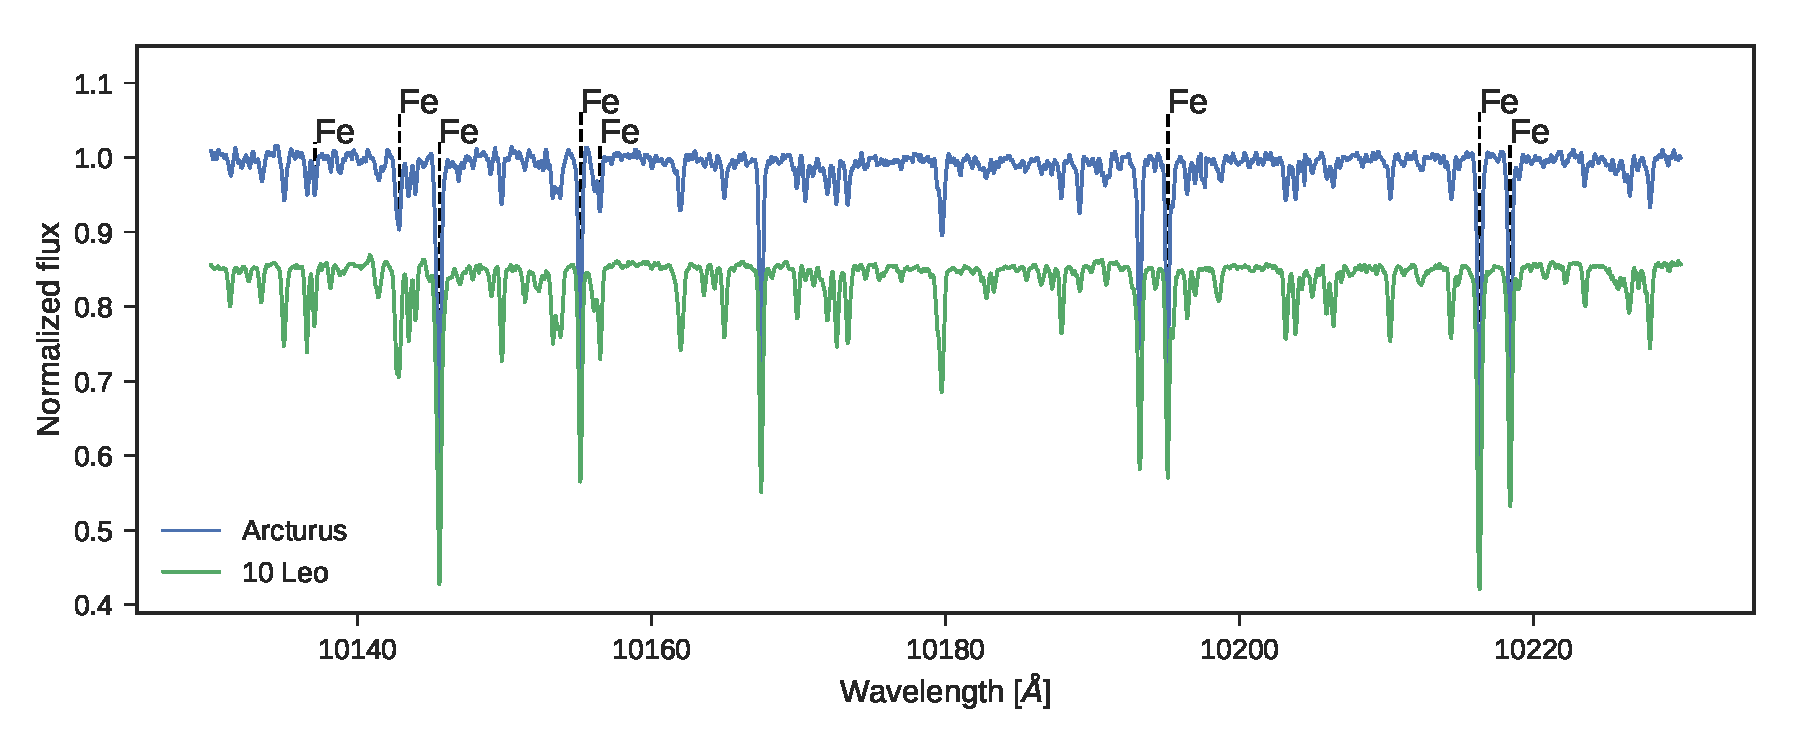
\includegraphics[width=1.0\linewidth]{figures/bothspectra.pdf}
    \caption{The spectrum of the two stars, in blue is Arcturus, and green is
             10 Leo. We mark the location of \ion{Fe}{I} lines in the region.}
    \label{fig:both}
\end{figure*}





\section{Refining the NIR line list}
\label{sec:refining_the_line_list}

Besides testing the line list at cooler effective temperatures with two K stars,
we also want to refine the line list. This includes identifying recurring
outliers, and lines which we are not able to measure, e.g. if a line is amidst a
forest of telluric lines. Hence, de-blending is nearly impossible. The first
step was to go back and have a second look at the solar atlas used in
\citet{Andreasen2016}. We removed 342 \ion{Fe}{I} lines and 13 \ion{Fe}{II}
lines in the process. Most of these were blended with other tellurics while a
few were blended with other stellar absorption lines. We are down to 84
\ion{Fe}{I} lines and 5 \ion{Fe}{II} lines. The \ion{Fe}{II} lines are used to
determine $\log g$ by imposing ionization balance with \ion{Fe}{I}. However, the
low number of \ion{Fe}{II} lines available is a concern, since the average
abundance of \ion{Fe}{II} is less trustworthy. One might fix $\log g$ during the
process of obtaining stellar parameters, but this has an impact on the other
derived parameters. It is better to leave $\log g$ free if possible, and either
make corrections at the end or change it to a value from a more reliable source.
This could for example be asteroseismology or from the parallaxes measured with
Gaia.


\section{Results}
\label{sec:results}

We derive the stellar atmospheric parameters in the same way as described in
\citet{Andreasen2016} using FASMA \citep{Andreasen2017a}. The EWs are measured
for both stars automatically with ARES \citep{Sousa2015a} and by hand with splot
in IRAF. We compare the derived stellar parameters from the two measured sets of
EWs.


\subsection{Arcturus}
\label{sec:arcturus}

Arcturus is one of the brightest stars on the night sky with a V magnitude of
-0.05 \citep{Ducati2002}. Hence it is a prime target for testing the line list
by \cite{Andreasen2016} with numerous measurements as mentioned above.

Lines blended with telluric were omitted from the analysis. The equivalent width
(EW) of rest of the lines were measured by hand using the splot function in
IRAF. In the atlas there exist both a summer observation set and a winter
observation set. This is in order to minimize the effect of tellurics at
different spectral regions. As many lines as possible were measured in both
sets. The EW measurements from the different data sets and method (automatic and
manual) can be seen in Fig.~\ref{fig:EWcomp}. Parameters were derived from the
manual measurements and from the automatic (using both the summer and winter
set). For all three sets parameters were derived with and without $\log g$
fixed. The derivation follows the procedure presented in \citet{Andreasen2016}
with removal 1 outlier iteratively after the minimization routine
\citep{Andreasen2017a} reach convergence. The final results are presented in
Tab.~\ref{tab:arcturus}.

\begin{figure}[tpb]
    \centering
    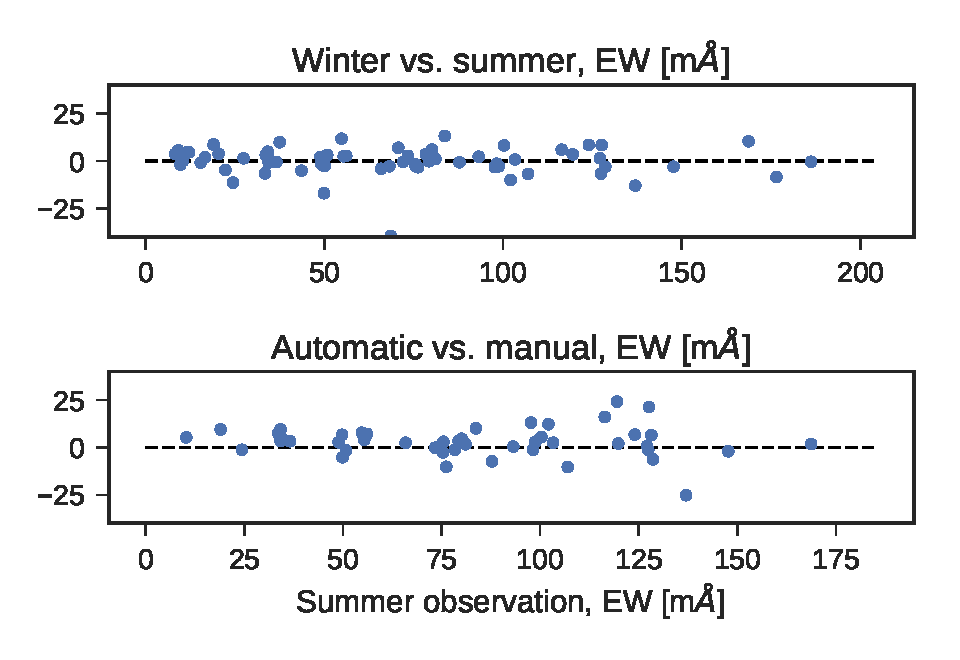
\includegraphics[width=1.0\linewidth]{figures/EWcomp.pdf}
    \caption{Top figure: compare the manual EWs measurement between the summer
             observations and winter observations. Bottom figure: Same as above,
             but with automatic measurements from ARES (summer) and manual
             measurements (summer).}
    \label{fig:EWcomp}
\end{figure}


\begin{table*}[htb!]
    \caption{The derived parameters for Arcturus with and without fixed surface
             gravity after 3$\sigma$ outlier removal. The literature values are
             a simple mean of all the available parameters on Simbad with the
             corresponding standard error. There is no microturbulence
             available, so we derived it using the empirical relation
             from \citet{Adibekyan2015} for each set of parameters.}
    \label{tab:arcturus}
    \centering
    \begin{tabular}{lllll}
      \hline\hline
                      & $T_\mathrm{eff}$ (K) &  $\log g$ (dex)  &   $\xi_\mathrm{micro}$ (km/s)   & [Fe/H] (dex)     \\
      \hline
        Literature    & $4306 \pm 100$       &  $1.69 \pm 0.32$ &    $1.92 \pm 0.15$              & $-0.54 \pm 0.11$ \\
      \hline
        IRAF          & $4380 \pm  79$       &  $0.64 \pm 0.33$ &    $1.14 \pm 0.09$              & $-0.49 \pm 0.07$ \\
        IRAF          & $4212 \pm  77$       &   1.69 (fixed)   &    $1.25 \pm 0.08$              & $-0.37 \pm 0.03$ \\
      \hline
        ARES (summer) & $4439 \pm  63$       &  $1.20 \pm 0.20$ &    $1.55 \pm 0.10$              & $-0.58 \pm 0.06$ \\
        ARES (summer) & $4348 \pm  75$       &   1.69 (fixed)   &    $1.58 \pm 0.09$              & $-0.53 \pm 0.03$ \\
        ARES (winter) & $4436 \pm  67$       &  $0.55 \pm 1.77$ &    $1.35 \pm 0.09$              & $-0.56 \pm 0.07$ \\
        ARES (winter) & $4233 \pm 109$       &   1.69 (fixed)   &    $1.43 \pm 0.09$              & $-0.49 \pm 0.04$ \\
      \hline
        Weighted mean & $4421 \pm  40$       &  $0.96 \pm 0.60$ &    $1.34 \pm 0.05$              & $-0.55 \pm 0.04$ \\
        Weighted mean & $4269 \pm  51$       &   1.69 (fixed)   &    $1.41 \pm 0.05$              & $-0.46 \pm 0.02$ \\
      \hline
    \end{tabular}
\end{table*}

We generally see good agreement between the derived parameters and the values
from the literature. The only parameter being difficult to measure is the
surface gravity due to the lack of \ion{Fe}{II} lines in the NIR. The
metallicity is very important to derive accurately, and we report good results
overall, but especially with the automatic measurements, compared to literature
values. For visualization the parameters are plotted (except
$\xi_\mathrm{micro}$) in Fig.~\ref{fig:arcturus}.

\begin{figure}[tpb]
    \centering
    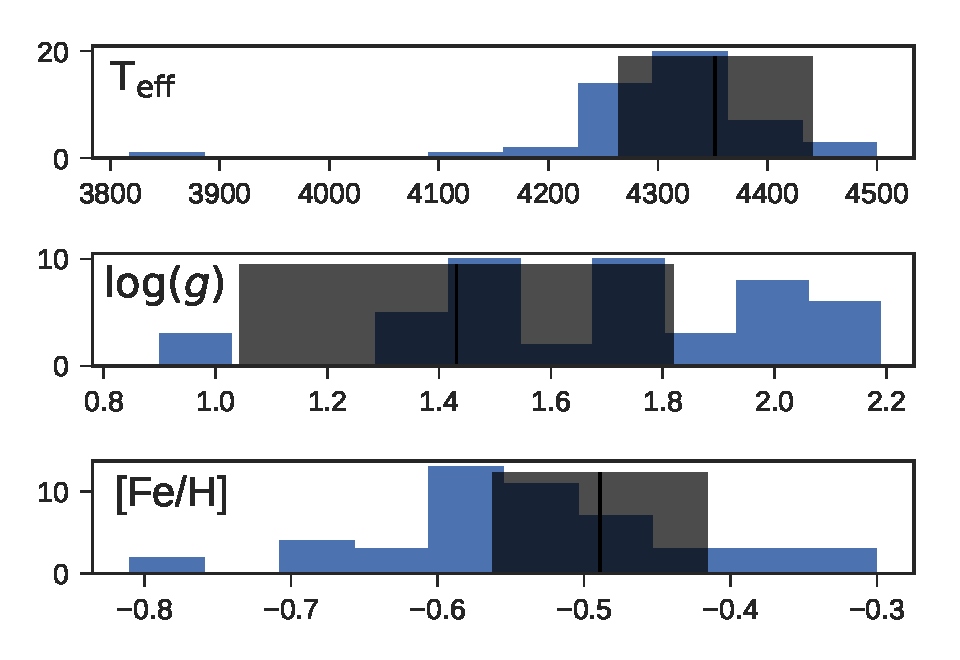
\includegraphics[width=1.0\linewidth]{figures/ArcturusParams.pdf}
    \caption{Histogram of the atmospheric stellar parameters of Arcturus (except
             $\xi_\mathrm{micro}$). The black vertical lines are the derived
             parameters, and the gray shaded area are the errors on the
             corresponding parameters.}
    \label{fig:arcturus}
\end{figure}



\subsection{10 Leo}
\label{sec:10Leo}

The approach for determining the atmospheric stellar parameters for 10 Leo is
identical as for Arcturus. The final reduced data is divided in YJ, H, and K
bands. We use ARES on each band separately. For the small gaps in the spectrum,
we simply set the value to 1, since the spectrum is already normalized. This
will also prevent ARES to measure any lines in these regions. The EWs from the
three regions are combined to one final line list used for the determination of
the parameters. We list the result in Tab.~\ref{tab:10Leo} alongside with a mean
of literature values taken from Simbad.

\begin{table*}[htb!]
    \caption{Same as Tab.~\ref{tab:arcturus}. The errors on $T_\mathrm{eff}$ and
             $\xi_\mathrm{micro}$ for the weighted mean with fixed $\log g$ are
             mathematically lower than reported, but we chose to set a lower
             limit. These errors are underestimated.}
    \label{tab:10Leo}
    \centering
    \begin{tabular}{lllll}
      \hline\hline
                     & $T_\mathrm{eff}$ (K) &  $\log g$ (dex)  &   $\xi_\mathrm{micro}$ (km/s)   & [Fe/H] (dex)     \\
      \hline
        Literature   & $4720 \pm  42$       &  $2.54 \pm 0.11$ &    $1.59 \pm 0.02$              & $ 0.00 \pm 0.03$ \\
      \hline
        IRAF         & $4835 \pm  85$       &  $2.41 \pm 0.41$ &    $1.28 \pm 0.08$              & $ 0.09 \pm 0.06$ \\
        IRAF         & $4768 \pm  88$       &   2.54 (fixed)   &    $1.20 \pm 0.08$              & $ 0.01 \pm 0.05$ \\
      \hline
        ARES         & $4805 \pm  98$       &  $2.42 \pm 0.61$ &    $1.23 \pm 0.10$              & $-0.01 \pm 0.07$ \\
        ARES         & $4768 \pm 105$       &   2.54 (fixed)   &    $1.20 \pm 0.10$              & $-0.01 \pm 0.06$ \\
      \hline
        Weighted mean& $4821 \pm  65$       &  $2.41 \pm 0.37$ &    $1.26 \pm 0.06$              & $ 0.04 \pm 0.05$ \\
        Weighted mean& $4768 \pm  69$       &   2.54 (fixed)   &    $1.20 \pm 0.06$              & $ 0.05 \pm 0.04$ \\
      \hline
    \end{tabular}
\end{table*}

Generally the derived parameters are in excellent agreement with the literature
values listed here. Surprisingly we are able to derive good $\log g$ values,
although quite large errors and consistently lower, compared to the results from
Arcturus.

A synthetic spectrum with the best parameters for both stars can be seen in
Fig.~\ref{fig:synth}. The region is the same as in Fig.~\ref{fig:both}. This is
for a visual representation of our solution. We did not use synthetic fitting
to obtain the parameters.

\begin{figure}[tpb]
    \centering
    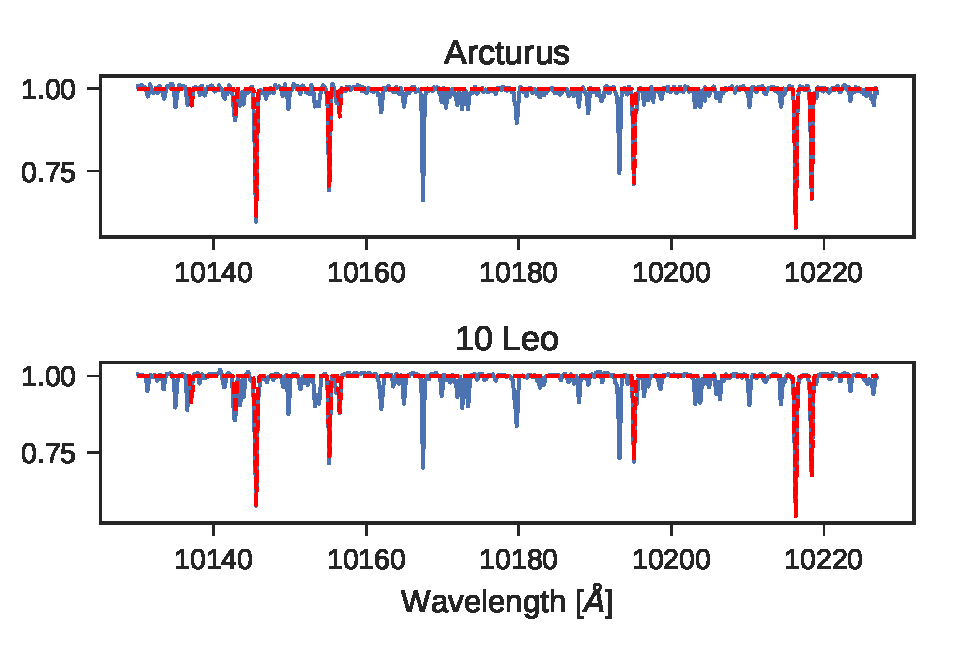
\includegraphics[width=1.0\linewidth]{figures/syntheticFit.pdf}
    \caption{Synthetic fit, red dashed curve, of both stars, blue curve, with
             the parameters from the weighted mean.}
    \label{fig:synth}
\end{figure}


\section{Discussion}
\label{sec:discussion}

\subsection{The role of $\log g$}

One of the most difficult atmospheric stellar parameters to get from a spectrum
is the surface gravity. Here we need the pressure sensitive ionized atoms such
as \ion{Fe}{II}. However, they are more sparse than neutral iron, \ion{Fe}{I}.
Hence the determination is challenging. This is true in the optical (give ref),
and even more in the NIR \citep[see e.g.][and this work]{Andreasen2016}. We seem
to get slightly better results when we fix the surface gravity when compared to
literature values. With the parallaxes from Gaia (give ref) we will have access
to accurate $\log g$, thus being able to have good $T_\mathrm{eff}$ and
$[\ion{Fe}/\ion{H}]$. We might also see a hint that the method work less well
for the most evolved stars (low $\log g$) as Arcturus. The weighted mean results
for 10 Leo are overlapping within the errorbars provided, which is not the case
for the $T_\mathrm{eff}$ of Arcturus, nor the $[\ion{Fe}/\ion{H}]$. However,
these values are all within the errorbars from the literature values. With the
coming spectral library from CARMENES (private comm. Amado, P.) we will have a
dwarf stars to test this method, which is what it is intended for.







\section{Conclusion}
\label{sec:conclusion}

Being able to successfully determine parameters for two early K giants, we are
now making the bridge for the line list towards cooler temperatures. The obvious
next step is the even colder M stars. Particular interesting are the M dwarfs
known to be prone forming rocky planets.





\begin{acknowledgements}

This work was supported by Funda\c{c}\~ao para a Ci\^encia e a Tecnologia (FCT)
through the research grants UID/FIS/04434/2013 and PTDC/FIS-AST/1526/2014.
N.C.S., and S.G.S. acknowledge the support from FCT through Investigador FCT
contracts of reference IF/00169/2012, and IF/00028/2014, respectively, and
POPH/FSE (EC) by FEDER funding through the program “Programa Operacional de
Factores de Competitividade - COMPETE”. E.D.M. acknowledge the support from FCT
in form of the fellowship SFRH/BPD/76606/2011. This work also benefit from the
collaboration of a cooperation project FCT/CAPES - 2014/2015 (FCT Proc 4.4.1.00
CAPES).

This research has made use of the SIMBAD database operated at CDS, Strasbourg
(France).

\end{acknowledgements}


\bibpunct{(}{)}{;}{a}{}{,}
\bibliographystyle{aa}
\bibliography{thesis}


\end{document}
